\chapter{Projectgrenzen}
In dit hoofdstuk worden de projectgrenzen toegelicht.
De afbakening van het project licht toe wat er wel en niet gemaakt binnen de context van de afstudeeropdracht.
Vervolgens wordt de definition of done beschreven om aan te tonen wanneer de opdracht voldaan is.
Daarna worden de randvoorwaarden van de afstudeeropdracht besproken.
\section{Afbakening}
Omdat het huidige Snakeware cloud platform erg groot is, is het belang dat afstudeeropdracht niet te groot wordt gemaakt zodat het afgerond kan worden binnen de af afstudeerperiode.
Het huidige Snakeware cloud platform bestaat uit 3 verschillende applicaties: De \gls{CMS}-API, de Snakeware cloud frontend, de webapplicatie.\\
\textbf{CMS-API}: Hier wordt de logica van het CMS uitgevoerd en de data verwerkt en opgehaald.
% De CMS API haalt de data op vanuit de database en toont dat op de \textbf{webapplicatie}.
% De data wordt aangepast via de \textbf{Snakeware cloud frontend}.\\
\textbf{Snakeware cloud frontend}: Hier mee kan de \textbf{klant} via een \gls{GUI} de content van de \textbf{webapplicatie} aanpassen.
Deze content wordt verwerkt en opgeslagen door middel van de \textbf{\gls{CMS}-API}.\\
\textbf{De webapplicatie}: hier wordt de content getoond die ingesteld is via de \textbf{Snakeware cloud interface}.
De \texbf{eindgebruiker} kan deze content inlezen via de publiekelijke bereikbare webapplicatie.
% \todo[inline]{aanpassen afbeelding kijken of er een UML diagram is die dit goed beschrijft, en bron postman workflows}
\begin{graphic}
    \captionsetup{type=figure}
    \caption{Producten die gemaakt worden tijdens de afstudeeropdracht}
    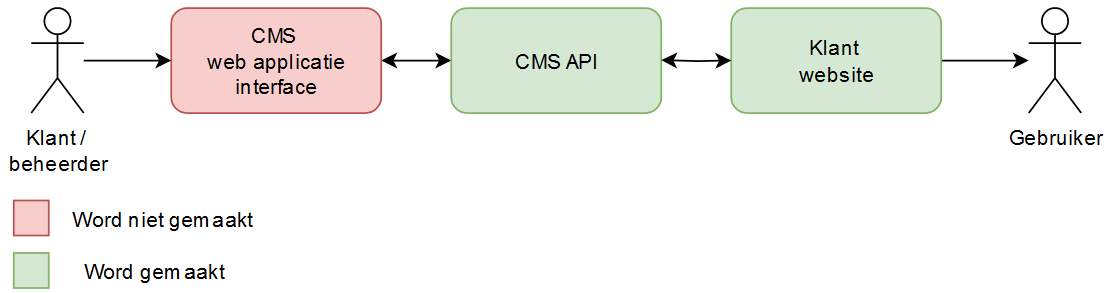
\includegraphics[scale=0.4]{ProductOverview}
    \label{fig:ProductOverview}
\end{graphic}
\whitespace
De opdracht wordt beperkt tot het ontwerpen en ontwikkelen van de \texbf{\gls{CMS}-API} en de webapplicatie.
Er is besloten om geen Snakeware cloud \gls{GUI} te maken om de scope en lengte van het project haalbaar te maken.
In figuur \ref{fig:ProductOverview} is te zien welke onderdelen gemaakt worden.
Om de user journeys te kunnen valideren worden ze getest door middel van postman workflows.
Er wordt wel een frontend applicatie gemaakt voor het renderen van de content, deze applicatie zal wel minimaal blijven.
\whitespace
% \textbf{Wel:}
% \whitespace
% - minimaal uitwerken van de \qw{must haves vanuit} de aanbevelingen van het onderzoek.
% \todo[inline]{gevoel dat hier nog extra dingen bij moeten staan.}
% \textbf{Niet:}
% \whitespace
% - een \gls{CMS} interface maken waarmee de klant content kan plaatsen voor de gebruiken.\\
% - de won't haves die van uit de aanbevelingen van het onderzoek komen uitwerken.
\section{Definition of done}
De definition of done is wanneer er een proof of concept \gls{CMS}-API en de daarbij behorende frontend is opgeleverd. 
Die voldoen aan de \qw{must have} eisen en wensen die uit het onderzoek zijn gekomen van de stakeholders.
Het systeem moet flexibel opgesteld worden, zodat in de toekomst extra functionaliteiten toegevoegd kunnen worden.
Daarnaast is het van belang dat de school documentatie met een voldoende wordt afgerond.
De verschillende documenten zijn: plan van aanpak, onderzoeksverslag en het technisch verslag.
Daarna moet het product en de presentatie met een voldoende afgerond worden.
\section{Randvoorwaarden}
Om het project goed af te kunnen ronden zijn er randvoorwaarden aan het project verbonden: \\
- Er is een werkplek nodig om alle werkzaamheden tijdens de afstudeerperiode te kunnen afronden.\\
- Er wordt een keer per week een afspraak gemaakt met de bedrijfsbegeleider en de docentbegeleider om de progressie te bespreken. \\ 
- de afstudeeropdracht moet afgerond worden binnen de duur van de afstudeerperiode. 
Dit is ongeveer 125 werkdagen en loopt van 18 november 2023 tot 5 april 2024.
